\begin{center}
    \begin{figure}[H]
        \centering

        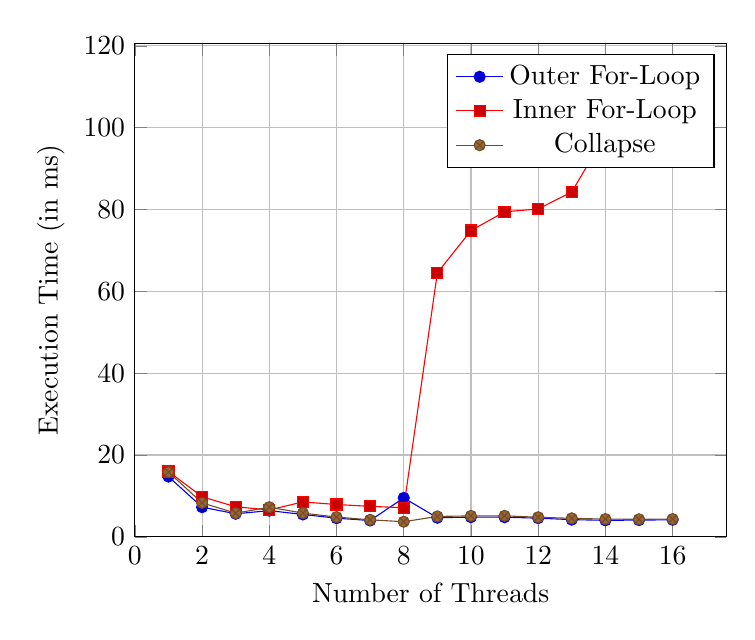
\begin{tikzpicture}
            \begin{axis}[
                title={},
                width=0.75\textwidth,
                xlabel={Number of Threads},
                ylabel={Execution Time (in ms)},
                xmin=0,
                ymin=0,
                grid=major
            ]
                \addplot coordinates {
                    (1,14.7211)(2,7.25495)(3,5.6363)(4,6.40325)(5,5.47325)(6,4.55525)(7,3.98965)(8,9.51975)(9,4.6724)(10,4.81735)(11,4.7994)(12,4.5654)(13,4.20095)(14,4.03585)(15,4.0938)(16,4.16465)
                };
                \addlegendentry{Outer For-Loop}

                \addplot coordinates {
                    (1,15.9672)(2,9.79695)(3,7.347)(4,6.57375)(5,8.53395)(6,7.9008)(7,7.455)(8,7.12075)(9,64.5109)(10,74.8451)(11,79.4215)(12,80.1279)(13,84.2831)(14,98.2654)(15,96.7823)(16,109.546)
                };
                \addlegendentry{Inner For-Loop}       

                \addplot coordinates {
                    (1,15.8111)(2,8.30245)(3,5.78465)(4,7.24315)(5,5.80145)(6,4.82905)(7,4.161)(8,3.69605)(9,4.9833)(10,5.11935)(11,5.1344)(12,4.7873)(13,4.5233)(14,4.33805)(15,4.2893)(16,4.3391)
                };
                \addlegendentry{Collapse}
            \end{axis}
        \end{tikzpicture}
        \caption{Grayscale Performance Tests dice\_large.png}
    \end{figure}
\end{center}